\documentclass{standalone}
\usepackage{pgfplots}
\usetikzlibrary{shapes.geometric, intersections, calc}
\pgfplotsset{compat=1.7}

\begin{document}
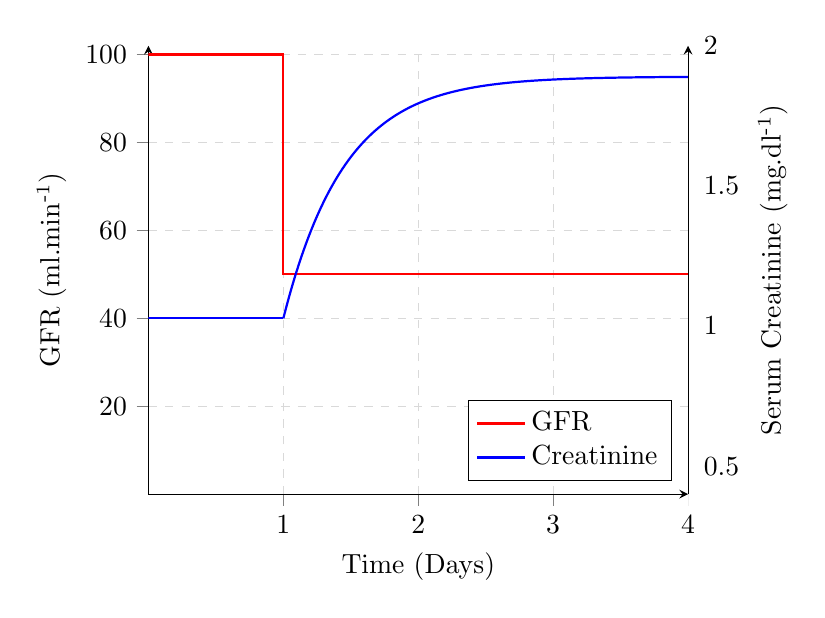
\begin{tikzpicture}[dot/.style={circle,inner sep=1pt,fill,label={#1},name=#1},
 extended line/.style={shorten >=-#1,shorten <=-#1},
 extended line/.default=10cm]

    \begin{axis}[
        axis x line=middle,
        axis y line=middle,
        grid = major,
        grid style={dashed, gray!30},
    	  x label style={at={(axis description cs:0.5,-0.1)},anchor=north},
	  y label style={at={(axis description cs:-0.1,.5)},rotate=90,anchor=south,precision=2},
        xmin=0,
        xmax= 4,
        ymin= 0,
        ymax= 102,
	 ylabel near ticks,
	xlabel near ticks,
        xlabel=Time (Days),
        ylabel=GFR (ml.min\textsuperscript{-1}),
        tick align=outside,
legend pos = south east,
legend cell align={left}]


	\coordinate (o) (0,0);
	\addplot[domain=0:1, red, thick,samples=500] {100};
	\draw[red, thick] (axis cs: 1,100) -- (axis cs: 1,50) -- (axis cs: 5,50);
\addlegendentry{GFR};

	\addplot[domain=1:5, blue, thick,samples=500] {55*(1-exp(-2.2*(x-1)))+40};
\addlegendentry{Creatinine};
	\draw[blue,thick] (axis cs: 0,40) -- (axis cs: 1,40);



\end{axis}
     \begin{axis}[
       xmin=0,xmax=2,ymin=0.4,ymax=2,
       axis x line=none,
 	axis y line=right,
ytick style={draw=none},
	extra y ticks={},
extra y tick labels = {},
       ylabel near ticks,
       ylabel={Serum Creatinine (mg.dl\textsuperscript{-1})}
     ]
     \end{axis}



\end{tikzpicture} 
\end{document}